\documentclass[12pt,letterpaper]{article}
\usepackage{amsmath}
\usepackage[margin=1in]{geometry}
\usepackage{fancyhdr}
\usepackage[utf8]{inputenc}
\usepackage{palatino}
\usepackage{microtype}
\usepackage{hyperref}
\usepackage{graphicx}
\usepackage{lastpage}
\usepackage[hang,small,margin=1in]{caption}
\usepackage{titlesec}

\renewcommand{\headrulewidth}{0pt}
\fancyfoot{}
\fancyfoot[C]{\sffamily Page \thepage\ of~\pageref{LastPage}}
\pagestyle{fancy}

\titleformat{\section}{\bfseries\MakeUppercase}{\arabic{\thesection}}{1em}{}
\titleformat{\subsection}{\bfseries}{\arabic{\thesection}.\arabic{\thesubsection}}{1em}{}
\titleformat{\subsubsection}{\itshape}{\arabic{\thesection}.\arabic{\thesubsection}.\arabic{\thesubsubsection}}{1em}{}

\setlength{\parindent}{0cm}
\setlength{\parskip}{1em}

\captionsetup[figure]{labelfont=it, font=it}
\captionsetup[table]{labelfont={it,sc}, font={it,sc}}

\hypersetup{colorlinks, linkcolor = black, citecolor = black, urlcolor = black}
\urlstyle{same}



\begin{document}

\fancyfoot{}
\begin{center}
  \hfill \\
  \vspace{4in}
  {\bf\Huge MTH351 Assignment 2} \\
  \vspace{2in}
  {\Large Soo-Hyun Yoo \\ 930569466 \\ April 22, 2015}
\end{center}

\newpage
\fancyfoot[C]{\sffamily Page \thepage\ of~\pageref{LastPage}}

\begin{enumerate}
  \item
    \begin{enumerate}
      \item Rearranging, we find:
        \begin{align*}
          \alpha &= \sqrt[m]{c} \\
          \alpha^m - c &= 0 \\
          f(x) &= \boxed{x^m - c}
        \end{align*}

      \item We need at least
        \begin{align*}
          |\alpha - c_n| &< \frac{1}{2^n} (b-a) \\
          10^{-10} &< \frac{1}{2^n} (b-a) \\
          2^n &< 10^{10}(b-a) \\
          n &> \boxed{\frac{\ln{10^{10}(b-a)}}{\ln 2}}
        \end{align*}
        iterations of bisection.

      \item If $f$ converges quadratically,
        \begin{align*}
          \lambda &\rightarrow \frac{-f''(\alpha)}{2f'(\alpha)} \\
                  &= \frac{-m(m-1)\alpha^{m-2}}{2m\alpha^{m-1}} \\
                  &= \boxed{\frac{1-m}{2\alpha}}.
        \end{align*}

      \item $\alpha = 2.6591$ was found after 4 iterations:
        {\scriptsize
          \begin{verbatim}
>> newtons(y,yp,3,1e-16,50)
   n          x                  f(x)              quad. ratio          lin. ratio
-------    -------------    -------------        -------------        -------------
   0    3.00000000e+00    3.10000000e+01
   1    2.71296296e+00    4.17207355e+00
   2    2.66072811e+00    1.18953238e-01        -6.33993045e-01        1.81979485e-01
   3    2.65914936e+00    1.05830296e-04        -5.78620802e-01        3.02241721e-02
   4    2.65914795e+00    8.40003622e-11        -5.64536804e-01        8.91265394e-04

ans =

    2.6591
          \end{verbatim}
        }

      \item The ratio is accurate to four digits: $\cfrac{1-4}{2\sqrt[4]{50}} = -0.5641 \approx {\tt -5.64536804e-01}$
    \end{enumerate}

  \item
    \begin{enumerate}
      \item Given $A = \frac{P}{r}(1-(1+r)^{-n})$, finding the highest possible
        $r$ is equivalent to finding the root of
        \[f(r) = \cfrac{P}{r}\left(1-(1+r)^{-n}\right) - A.\]
        In order to use Newton's method, we also need
        \[f'(r) = -\cfrac{P}{r^2}\left(1-(1+r)^{-n}\right) + \cfrac{P}{r}\left(n(1+r)^{-n-1}\right).\]

      \item With $x_0 = 0.04$, $\boxed{r \approx 0.0284}$. This lower allowable
        interest rate is consistent with the lower rate of payment per year.
        The script is as follows:
        {\footnotesize
          \begin{verbatim}
function r = annuity(A, P, n)
    f  = @(r) P/r*(1- (1+r)^-n) - A;
    fp = @(r) -P/r^2*(1- (1+r)^-n) + P/r*n*(1+r)^(-n-1);
    x0 = .04;
    tol = 1e-16;
    r = newtons(f,fp,x0,tol,50)
end
          \end{verbatim}
        }
    \end{enumerate}

  \item
    \begin{enumerate}
      \item The multiplicity appears to be odd. It is unclear whether or not it
        is bigger than 1.
        \begin{figure}[!h]
          \centering
          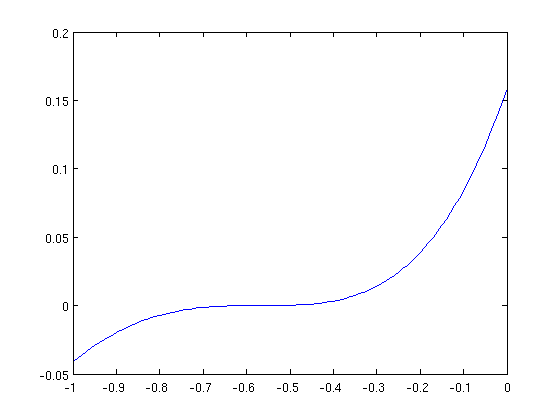
\includegraphics[width=0.6\textwidth]{3a.png}
        \end{figure}

      \item For $f'(x) = -(e^x+1)(\cos(x+e^x)-1)$, Newton's method converges
        linearly. The linear ratio is around $0.66$, or $\frac23$, which means
        the multiplicity $m = 3$.
      \item --
    \end{enumerate}
\end{enumerate}

\end{document}
